%REF:
%Section 3:
%How reliable are the uncertainties in table 3? Some uncertainties seem small to me. It is also surprising to see how constant these uncertainties are in absolute value from region to region for a quite variable set of input spectra. As one example: it does not make much sense to me that the absolute uncertainty on the 6.2 band in region #1 and region #8 are identical. The uncertainties on the smaller bands like the 12.0 um band are small (e.g. region 9 or the bulge). You yourself (implicitly) cast a doubt on the uncertainties when you discuss the outliers in figure 12 (sect 4.3).

The final processed IRS spectra are shown in  Figure \ref{PAHFITplots}, except for the nucleus, discussed in Section~\ref{sect:nucleus}.
All of the main PAH features, including the 6.2, 7.7, 8.6 and 11.3~$\mu$m bands, 
are clearly visible for all the regions shown here.
The IRS spectra also show atomic line emission such as [Ar~{\sc ii}], [Ar~{\sc iii}], [S~{\sc iii}], [S~{\sc iv}], [Ne~{\sc ii}], [Ne~{\sc iii}] 
and molecular H$_{2}$ emission at 12.3~$\mu$m. Some of the spectra display a contribution to the continuum from starlight emission.


\begin{figure*}
\centering
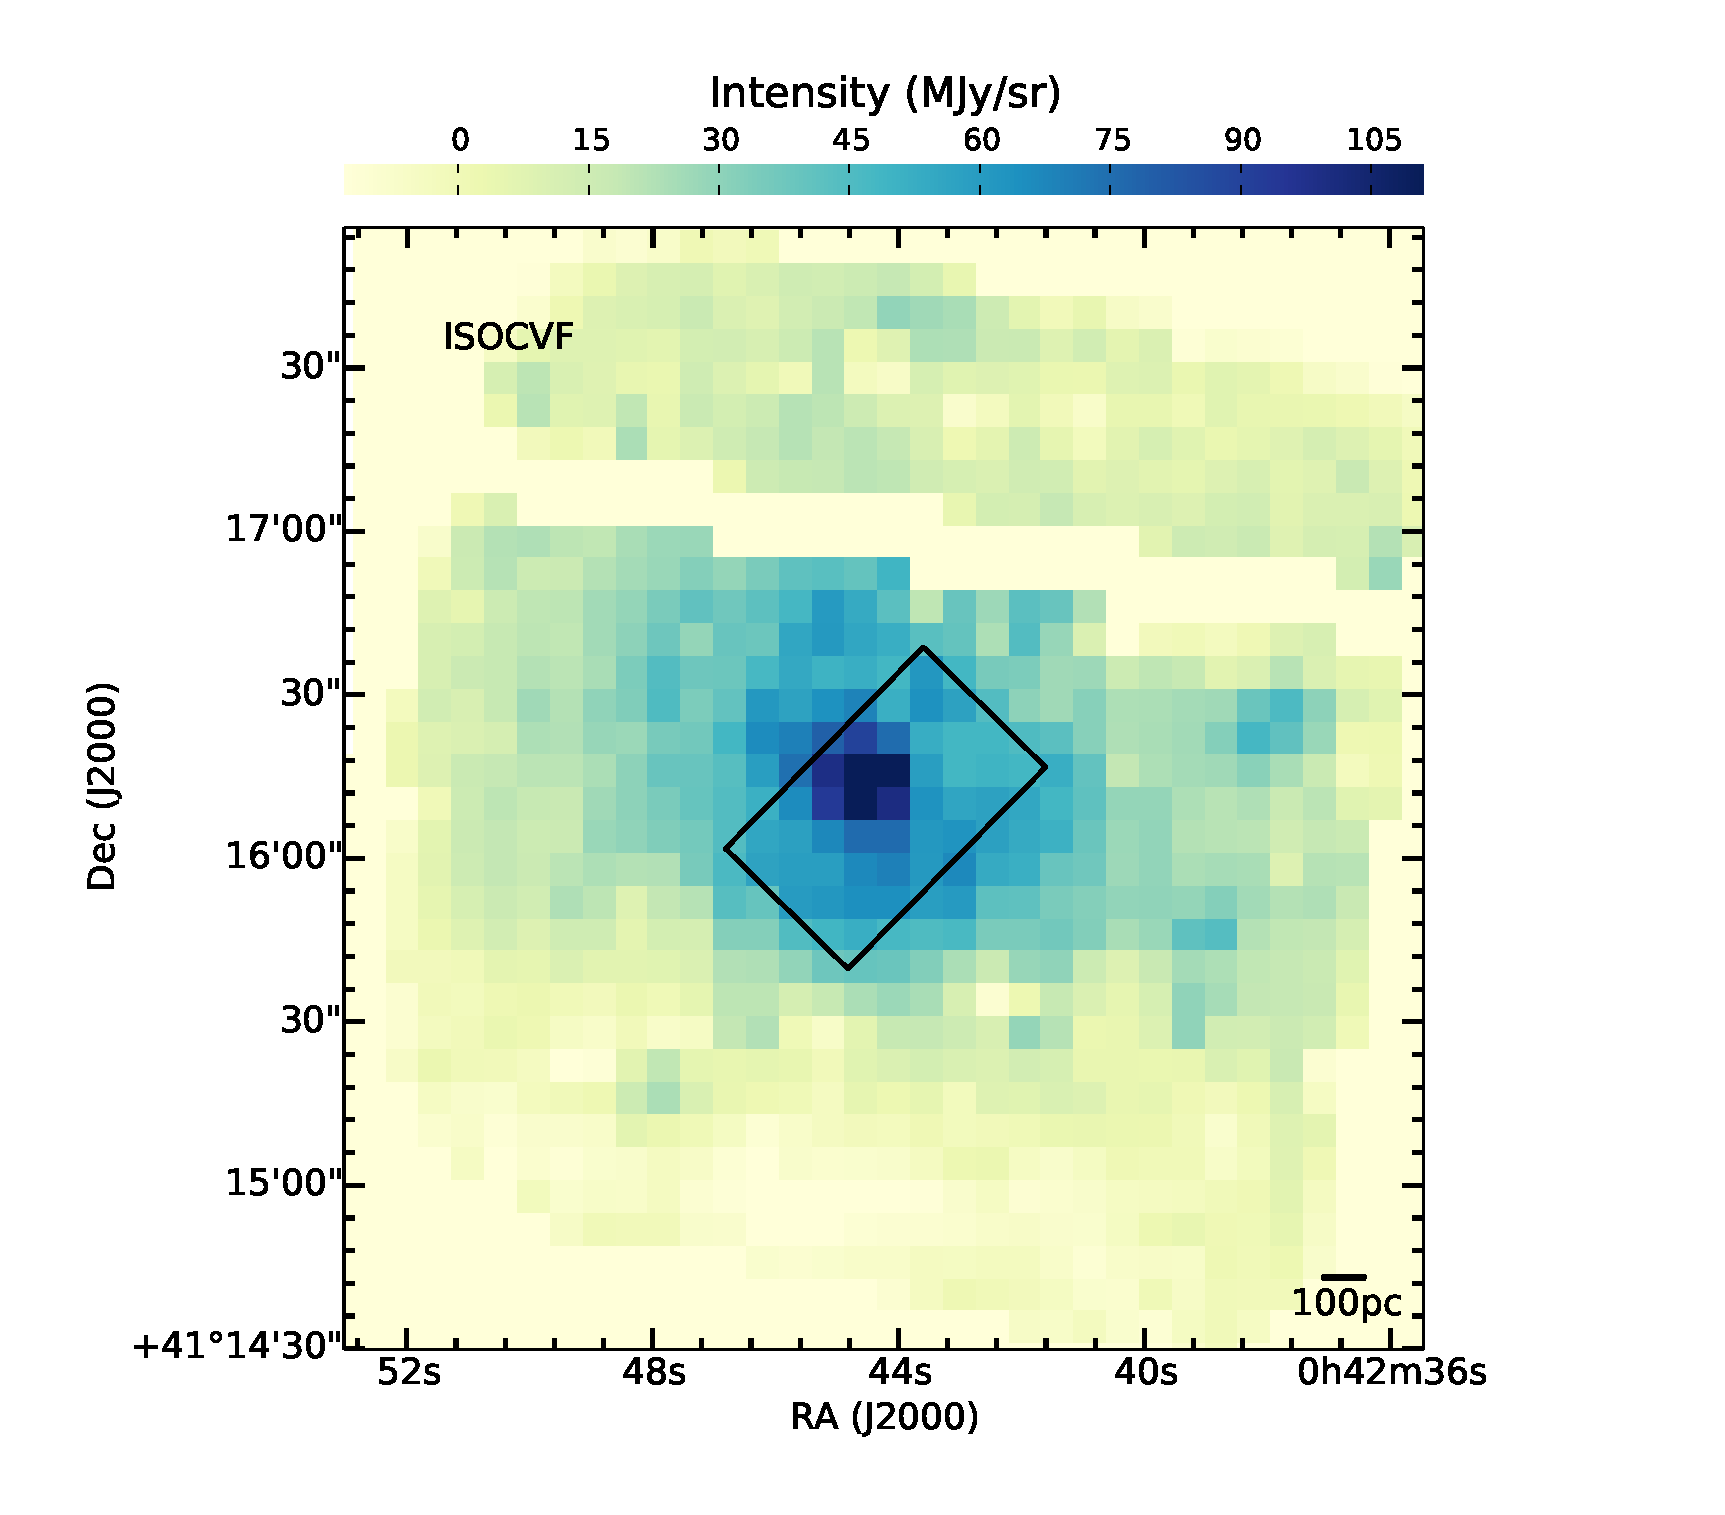
\includegraphics[scale=0.45]{./fig5.eps}
 \caption{Observed IRS spectra and detailed PAHFIT decompositions (see Section~\ref{sect:pahfit}). Regions are labeled in each panel.
Black squares show the observed data, and red, blue, light blue, pink and green lines represent the modelled
dust continua, PAH features, atomic lines, starlight continuum and the fit respectively. The black line shows the total modelled continuum. 
Vertical scales differ in different panels. Spectra from the nucleus and NGC 206 are not shown here.
}
\label{PAHFITplots}
\end{figure*}


\subsection{ISOCAM versus IRS}
\label{sect:iso_vs_irs}

As mentioned in the Introduction, based on ISOCAM observations of four regions in M31, \citet{1998Cesarsky} reported 
suppression of the common 6--8~$\mu$m PAH bands and a strong 11.3$\mu$m PAH band.
The 11.3~$\mu$m band profile was found to vary from region to region.  
In addition, \citet{Pagani_1999} confirmed that the star-forming ring in M31 shows very weak PAH emission in the 6 to 8~$\mu$m region. 
However, the IRS spectra presented here, except the nucleus, do not show such unusual behaviour (Figure~\ref{PAHFITplots}). 
Indeed all regions, except the nucleus, show a normal mid-infrared spectrum similar to other nearby starforming galaxies. 

Until 2005, ISOCAM-CVF data were not properly background subtracted and they were contaminated with zodiacal emission and stray light. 
Differential spectra between regions of relatively strong and weak emission were previously used to overcome this problem 
(more details about the differential spectra are given by \citealt{1998Cesarsky}, \citealt{Pagani_1999}). 
In 2005, all ISOCAM-CVF data were reprocessed  and corrected for the zodiacal emission \citep{Boulanger_F_2005}. 
We obtained newly-processed ISOCAM spectra from three regions in our IRS sample (see Section~\ref{sect:iso_data}) 
in order to compare them with the corresponding IRS spectra.
Figure~\ref{ISOnIRS} shows that although the relative feature intensities  in the IRS and ISOCAM 
spectra differ in detail, the spectral shapes are almost identical;
the re-processed ISOCAM data do not agree with the previous differential spectra.
Neither the bulge nor Region 9 shows any depletion in  6 to 8~$\mu$m features as described by \citet{1998Cesarsky}. 
The new ISOCAM reduction appears to eliminate the discrepancies between ISOCAM and IRS, resulting
in less `strange' infrared spectra for M31. For the remainder of this work, we discuss only the IRS spectra.



\begin{figure}
\centering
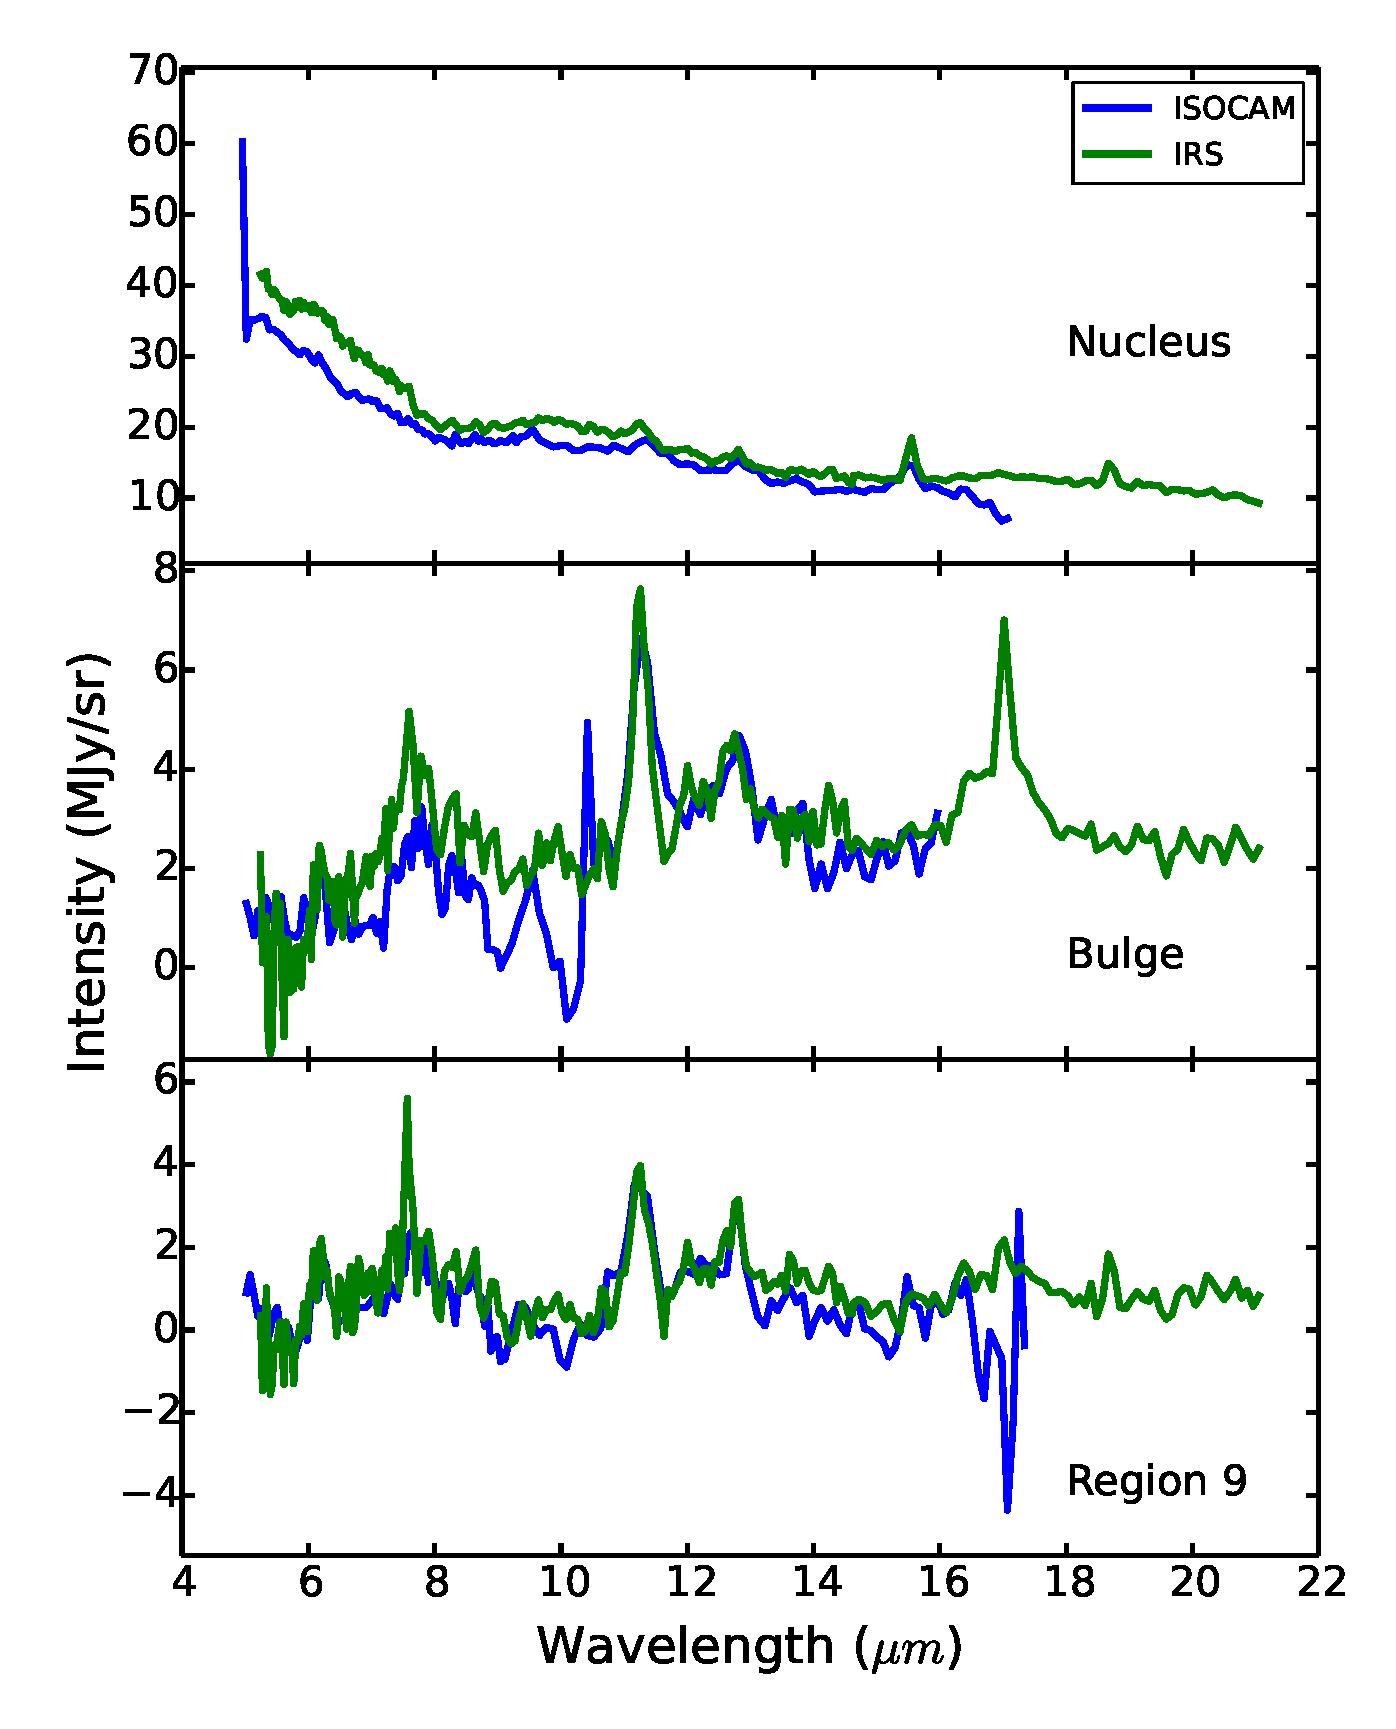
\includegraphics[scale=0.35]{./fig6.eps}
\caption{ Comparison of  IRS and re-processed ISOCAM spectra for the Nucleus (top), Bulge (middle) and Region 9 (bottom) in M31.}
\label{ISOnIRS}
\end{figure}



\subsection{PAHFIT}
\label{sect:pahfit}
The PAH features in  IRS spectra are often blended with neighbouring PAH features and atomic lines. 
Therefore measuring the strength of PAH features is difficult.  To achieve this task a tool called PAHFIT, introduced by \citet{Smith:2007lr}, was used. 
PAHFIT is an IDL  based tool designed for decomposing {\em Spitzer} IRS low-resolution spectra of PAH emission sources.
PAHFIT uses six main components to fit the surface brightness. These are starlight continuum, featureless thermal dust continuum, 
pure rotational lines of H$_2$, fine-structure lines, dust emission features and dust extinction. The starlight is represented by  blackbody 
emission at a fixed temperature of 5000~K, and the dust continuum is represented by 8 modified blackbodies (emissivity proportional to $\nu^2$)  
at fixed temperatures of 35, 40, 50, 65, 90, 135, 200, and 300~K. The final fit obtained with PAHFIT does not necessarily use
all eight dust components.
The infrared extinction is considered as a combination of a power law plus silicate absorption features with peaks at 9.7 and 18~$\mu$m. 
Line features are represented by Gaussian profiles with widths set by the instrumental resolution
and dust features are represented by Drude profiles; more details about PAHFIT are given by \citet{Smith:2007lr}.


Initial attempts at fitting the spectra with PAHFIT showed that some components were negligible, and
to avoid over-fitting we re-ran the fits without these components.
None of the IRS spectra shows significant silicate absorption around 9.7 or 18~$\mu$m, and the extinction calculated by PAHFIT 
was almost zero for all the initial fits. Except for four regions (the bulge, Region 5, Region 6 and Region 8),
the starlight contribution is also negligible.
We adjusted the PAHFIT input parameters to fix extinction to zero for all regions and starlight to zero for all but the four regions above.
Typically only two or three thermal dust components had significant power in our fits, but we did not fix the unused components to zero.
Regions 3 and 9 were found to have very low dust continuum emission compared to other spectra,
possibly because of noisy data at short wavelengths. However the other features in these spectra appear to
be fit correctly. The spectrum of the nucleus shows silicate emission, which is not included in PAHFIT;  
our modifications of PAHFIT to analyze this spectrum are discussed in see Section~\ref{sect:nucleus}.

\begin{table*}
 \centering
 \begin{minipage}{200mm}
\caption{PAH Emission Line Strengths$^a$}
{\scriptsize
  \begin{tabular}{l c c  c  c  c  c  c  c  c  c c }
\hline
    {Region }&{5.7 $\mu$m  }&{6.2 $\mu$m  }&{7.7 $\mu$m$^b$  }&{8.3 $\mu$m  }&{8.6 $\mu$m  }&{10.7 $\mu$m  }&{11.3 $\mu$m$^b$  }&{12.0 $\mu$m  }&{12.7 $\mu$m$^b$  }&{17.0 $\mu$m$^b$  } \\
 \hline
  %  Pub_ID  PAH5.7flx  PAH6.2flx  PAH7.7flx  PAH8.3flx  PAH8.6flx  PAH10.7flx  PAH11.3flx  PAH12.0flx  PAH12.7flx  PAH17.0flx 
%  None  1e-15W/m2  1e-15W/m2  1e-15W/m2  1e-15W/m2  1e-15W/m2  1e-15W/m2  1e-15W/m2  1e-15W/m2  1e-15W/m2  1e-15W/m2 
       Bulge  & \dots & $1.32 \pm 0.08$ & $7.7 \pm 0.6$ & $1.1 \pm 0.2$ & $0.7 \pm 0.1$ & $0.07 \pm 0.03$ & $1.85 \pm 0.08$ & $0.49 \pm 0.05$ & $1.02 \pm 0.09$ & $1.39 \pm 0.04$\\
    Region 1  & $0.36 \pm 0.05$ & $1.20 \pm 0.04$ & $3.8 \pm 0.2$ & $0.46 \pm 0.04$ & $0.50 \pm 0.03$ & $0.08 \pm 0.01$ & $1.18 \pm 0.02$ & $0.32 \pm 0.02$ & $0.54 \pm 0.02$ & $0.58 \pm 0.02$\\
    Region 2  & $0.27 \pm 0.03$ & $1.10 \pm 0.03$ & $3.7 \pm 0.2$ & $0.33 \pm 0.04$ & $0.70 \pm 0.03$ & $0.053 \pm 0.008$ & $1.13 \pm 0.02$ & $0.23 \pm 0.01$ & $0.51 \pm 0.03$ & $0.51 \pm 0.02$\\
    Region 3  & $0.3 \pm 0.1$ & $0.9 \pm 0.1$ & $3.9 \pm 0.6$ & $0.7 \pm 0.1$ & $0.3 \pm 0.1$ & \dots & $0.68 \pm 0.07$ & $0.21 \pm 0.05$ & $0.47 \pm 0.07$ & $0.45 \pm 0.04$\\
    Region 4  & $0.14 \pm 0.04$ & $0.56 \pm 0.03$ & $2.1 \pm 0.2$ & $0.26 \pm 0.04$ & $0.41 \pm 0.03$ & $0.029 \pm 0.008$ & $0.70 \pm 0.02$ & $0.12 \pm 0.01$ & $0.31 \pm 0.02$ & $0.44 \pm 0.02$\\
    Region 5  & \dots & $0.24 \pm 0.04$ & $0.79 \pm 0.07$ & $0.12 \pm 0.04$ & $0.21 \pm 0.03$ & $0.032 \pm 0.008$ & $0.45 \pm 0.02$ & $0.09 \pm 0.01$ & $0.22 \pm 0.01$ & $0.33 \pm 0.04$\\
    Region 6  & \dots & $0.26 \pm 0.03$ & $0.8 \pm 0.2$ & $0.10 \pm 0.03$ & $0.13 \pm 0.03$ & $0.029 \pm 0.008$ & $0.38 \pm 0.02$ & $0.07 \pm 0.01$ & $0.16 \pm 0.01$ & $0.29 \pm 0.02$\\
    Region 7  & $0.21 \pm 0.03$ & $0.62 \pm 0.03$ & $2.0 \pm 0.2$ & $0.30 \pm 0.04$ & $0.45 \pm 0.03$ & $0.058 \pm 0.008$ & $0.77 \pm 0.02$ & $0.18 \pm 0.01$ & $0.37 \pm 0.03$ & $0.47 \pm 0.04$\\
    Region 8  & \dots & $0.09 \pm 0.04$ & $0.22 \pm 0.07$ & $0.09 \pm 0.04$ & $0.10 \pm 0.03$ & $0.051 \pm 0.009$ & $0.16 \pm 0.02$ & \dots & \dots & $0.15 \pm 0.02$\\
    Region 9  & \dots & $1.3 \pm 0.1$ & $4.4 \pm 0.6$ & $0.9 \pm 0.1$ & $0.5 \pm 0.1$ & $0.09 \pm 0.03$ & $1.32 \pm 0.07$ & $0.51 \pm 0.05$ & $0.83 \pm 0.07$ & $0.6 \pm 0.1$\\

 \hline
 \label{PAHlinetable}
\end{tabular}\\
{$^a$Units are 10$^{-15}$~W~m$^{-2}$.\\
$^b$PAH complexes, as described in text.}
}
\end{minipage}
\end{table*}



\begin{table*}
 \centering
 \begin{minipage}{200mm}
 
\caption{PAH Emission Line Equivalent Widths$^a$}
 {\scriptsize
  \begin{tabular}{l c c  c  c  c  c  c  c  c  c c }
  \hline 
     {Region }&{5.7 $\mu$m  }&{6.2 $\mu$m  }&{7.7 $\mu$m$^b$  }&{8.3 $\mu$m  }&{8.6 $\mu$m  }&{10.7 $\mu$m  }&{11.3 $\mu$m$^b$  }&{12.0 $\mu$m  }&{12.7 $\mu$m$^b$  }&{17.0 $\mu$m$^b$  } \\
 \hline
 %  Pub_ID  PAH5.7eqw  PAH6.2eqw  PAH7.7eqw  PAH8.3eqw  PAH8.6eqw  PAH10.7eqw  PAH11.3eqw  PAH12.0eqw  PAH12.7eqw  PAH17.0eqw 
%  None  micron  micron  micron  micron  micron  micron  micron  micron  micron  micron 
       Bulge  & \dots & $1.2 \pm 0.2$ & $4.1 \pm 0.4$ & $0.51 \pm 0.07$ & $0.30 \pm 0.06$ & $0.03 \pm 0.01$ & $0.78 \pm 0.04$ & $0.22 \pm 0.02$ & $0.49 \pm 0.05$ & $1.16 \pm 0.04$\\
    Region 1  & $0.39 \pm 0.08$ & $1.2 \pm 0.1$ & $3.4 \pm 0.3$ & $0.43 \pm 0.04$ & $0.47 \pm 0.04$ & $0.09 \pm 0.01$ & $1.45 \pm 0.04$ & $0.43 \pm 0.03$ & $0.76 \pm 0.04$ & $1.26 \pm 0.05$\\
    Region 2  & $0.28 \pm 0.04$ & $1.02 \pm 0.06$ & $3.4 \pm 0.2$ & $0.32 \pm 0.04$ & $0.70 \pm 0.04$ & $0.07 \pm 0.01$ & $1.58 \pm 0.04$ & $0.35 \pm 0.02$ & $0.85 \pm 0.05$ & $1.33 \pm 0.06$\\
    Region 3  & $4.3 \pm 2.3$ & $8.3 \pm 2.3$ & $18.5 \pm 4.2$ & $2.8 \pm 0.8$ & $0.9 \pm 0.5$ & \dots & $2.1 \pm 0.3$ & $0.7 \pm 0.2$ & $1.6 \pm 0.3$ & $2.4 \pm 0.3$\\
    Region 4  & $0.28 \pm 0.09$ & $1.0 \pm 0.1$ & $3.7 \pm 0.4$ & $0.48 \pm 0.07$ & $0.77 \pm 0.07$ & $0.07 \pm 0.02$ & $1.67 \pm 0.06$ & $0.31 \pm 0.04$ & $0.82 \pm 0.06$ & $1.65 \pm 0.08$\\
    Region 5  & \dots & $0.12 \pm 0.03$ & $0.61 \pm 0.07$ & $0.10 \pm 0.03$ & $0.20 \pm 0.03$ & $0.05 \pm 0.01$ & $0.77 \pm 0.04$ & $0.17 \pm 0.03$ & $0.50 \pm 0.04$ & $1.6 \pm 0.2$\\
    Region 6  & \dots & $0.10 \pm 0.04$ & $0.6 \pm 0.2$ & $0.10 \pm 0.04$ & $0.14 \pm 0.03$ & $0.05 \pm 0.01$ & $0.77 \pm 0.05$ & $0.15 \pm 0.03$ & $0.42 \pm 0.05$ & $1.7 \pm 0.1$\\
    Region 7  & $0.32 \pm 0.05$ & $0.86 \pm 0.06$ & $2.2 \pm 0.1$ & $0.44 \pm 0.06$ & $0.69 \pm 0.06$ & $0.12 \pm 0.02$ & $1.81 \pm 0.07$ & $0.48 \pm 0.05$ & $1.08 \pm 0.09$ & $2.2 \pm 0.3$\\
    Region 8  & \dots & \dots & $0.10 \pm 0.05$ & $0.09 \pm 0.04$ & $0.10 \pm 0.03$ & $0.09 \pm 0.02$ & $0.30 \pm 0.04$ & \dots & \dots & $0.62 \pm 0.08$\\
    Region 9  & \dots & $\left(2.4 \pm 1.1\right) \times 10^{2}$ & $\left(1.4 \pm 0.4\right) \times 10^{2}$ & $15.5 \pm 5.6$ & $7.9 \pm 2.8$ & $0.5 \pm 0.2$ & $6.8 \pm 1.1$ & $2.3 \pm 0.6$ & $3.5 \pm 0.8$ & $2.2 \pm 0.8$\\

 \hline
 \label{EQW}
\end{tabular}\\
{$^a$Units are $\mu$m.\\
$^b$PAH complexes, as described in text.\\
Continuum for Regions 3 and 9 is very weak.  Equivalent widths are highly uncertain and not considered in the analysis (see Section~\ref{sect:data_analysis}).}
}
\end{minipage}
\end{table*}



\subsection{PAH features}
\label{sect:pah}

PAHFIT returns fluxes and equivalent widths (EQWs) of PAH features, which are given in Tables~\ref{PAHlinetable} and \ref{EQW}. 
For easier comparison with previous work, the tables give measurements for the 7.7, 11.3, 12.7 and 17.0~$\mu$m PAH complexes
as defined by \citet{Smith:2007lr}, as computed from the individual constituent features measured by PAHFIT.
The intensities of the features do not include any contribution from the continuum, but the equivalent width computed by
\begin{equation}
{\rm EQW}=\int \frac{I_{\nu,{\rm feature}}}{I_{\nu, {\rm cont}}} \,d\lambda,
\end{equation}
is a measure of the ratio of the continuum emission ($I_{\nu, {\rm cont}} $) to the line strength 
($I_{\nu,{\rm feature}}=I_{\nu} =- I_{\nu, {\rm cont}})$. 
The continuum emission is mainly from dust grains, much larger than PAH molecules. Hence, by studying EQWs of PAHs, 
we can study how the PAHs compete with the dust grains in the mid-infrared wavelengths.  PAHFIT returns the EQWs for each PAH 
feature, we calculated the uncertainties using a Monte-Carlo method. In that method, for each region, PAHFIT was run 500 times on 
randomly generated data points  normally distributed within the uncertainties of the spectrum. PAHFIT returned 500 EQWs for each 
PAH feature, and the standard deviation of EQWs for a given feature was taken as its uncertainty. 
The EQWs from Regions 3 and 9 were removed from further analysis because the negligible dust continuum for these spectra makes
the EQWs highly uncertain.


\subsection{Atomic line features}
\label{sect:atomic}



\begin{figure}
\centering
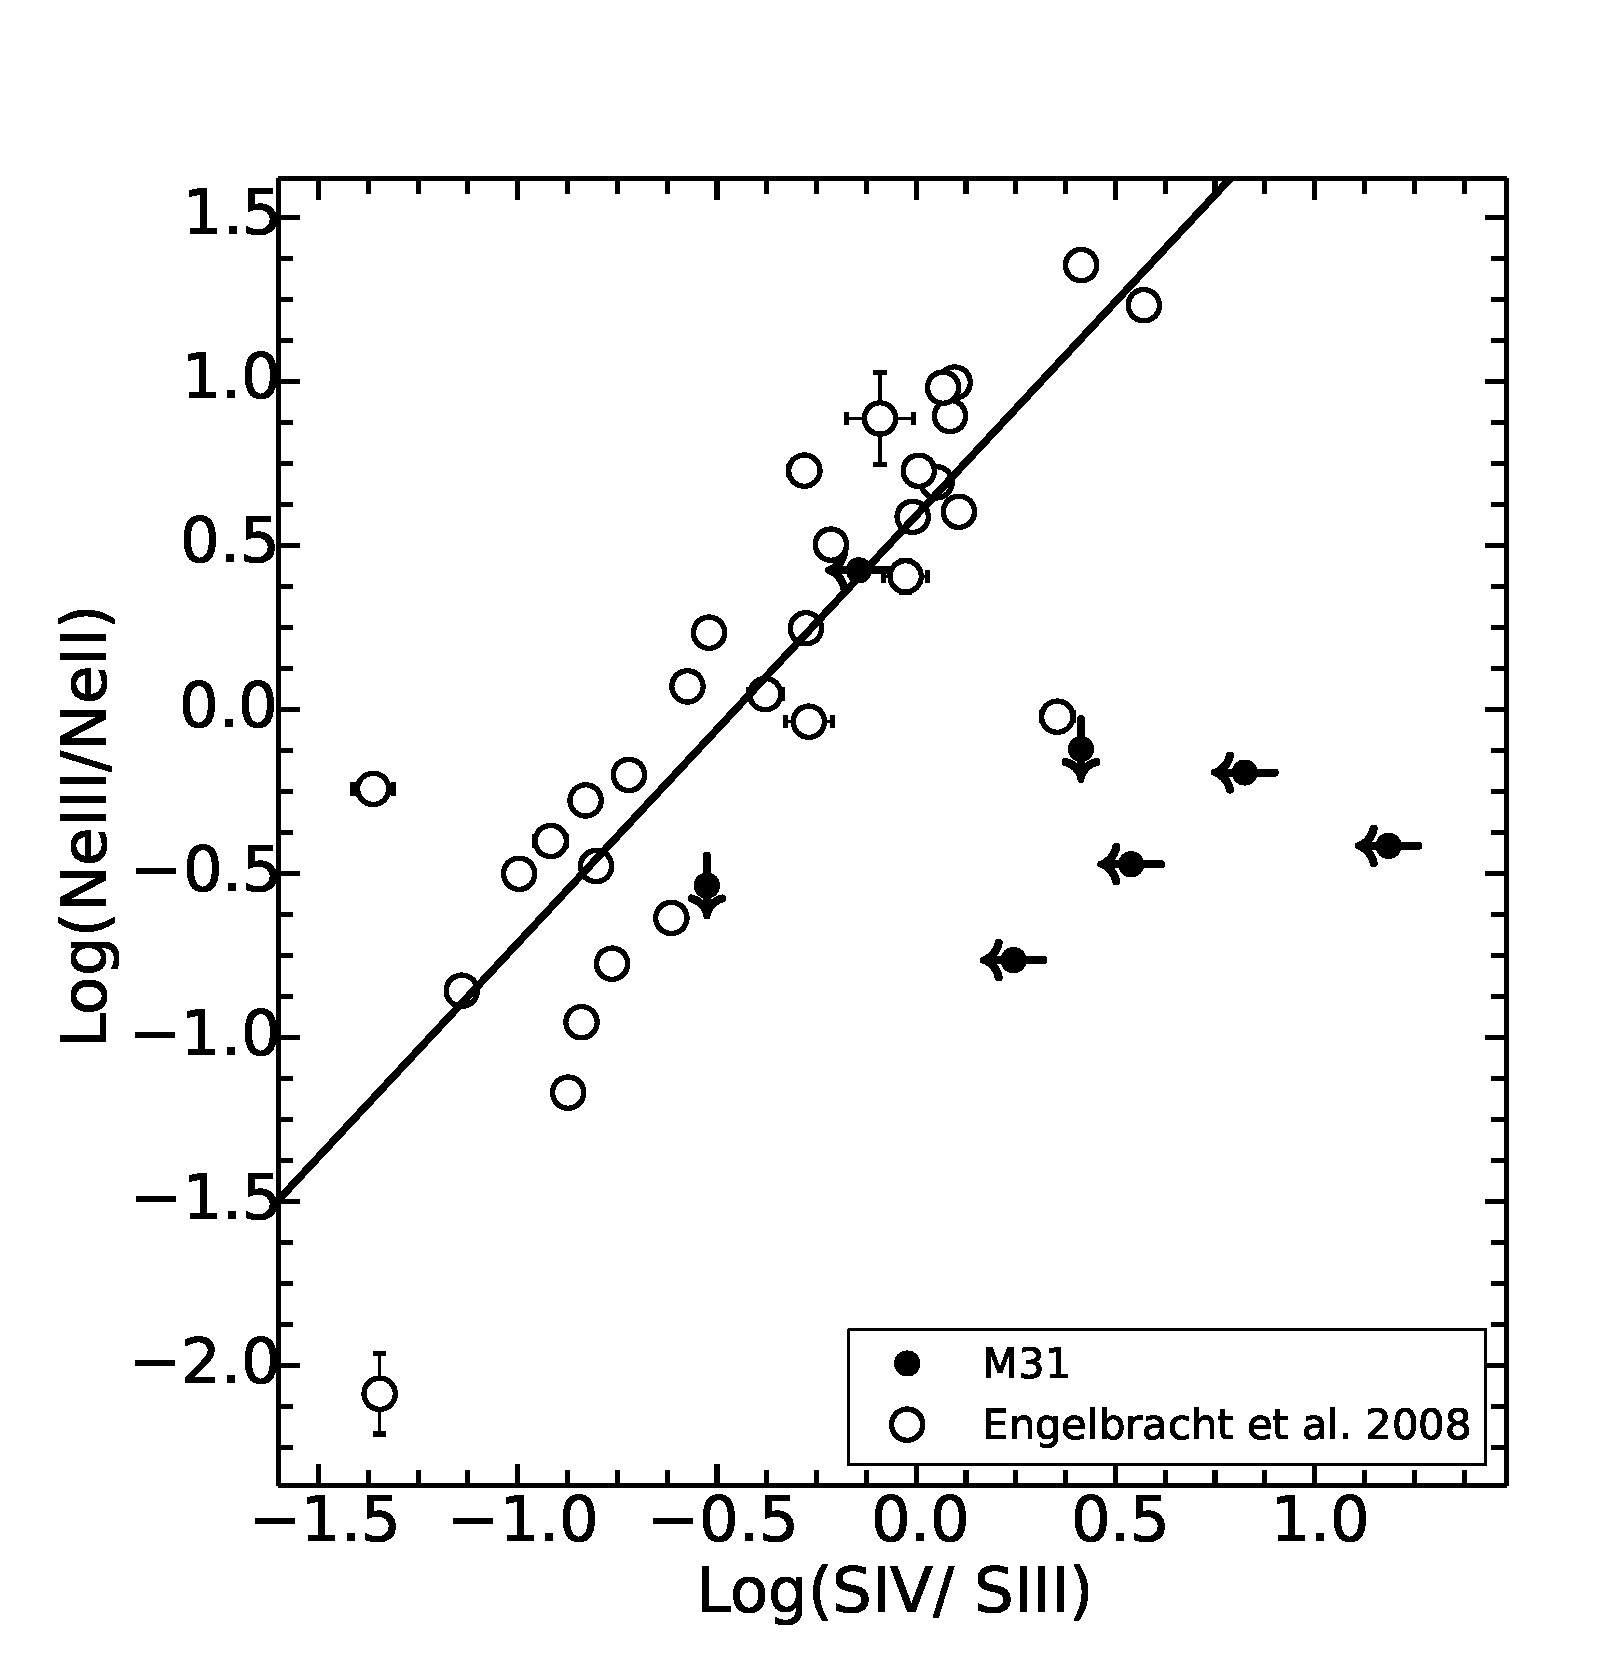
\includegraphics[scale=0.27]{./fig7.eps}
\caption{ Log([Ne~{\sc iii}]/[Ne~{\sc ii}])  vs log([S~{\sc iv}]/[S~{\sc iii}])  for the M31 regions in our sample (black dots) and  the starburst sample from \citet{Engelbracht_2008} (open dots). The straight line is the line of best fit for the starburst sample.
Upper limits are $3\sigma$.
}
\label{SvsNe}
\end{figure}

PAHFIT also returns the line strengths and uncertainties for atomic lines, listed in Table~\ref{Atomic}.
Not all lines were detected by PAHFIT, so we calculated upper limits for non-detected lines.%
\footnote{To find  the upper limits for the flux of missing atomic lines, we assumed the line to be a 
Gaussian profile with a FWHM as given by PAHFIT. The peak intensity was taken to be 3 times the RMS, where RMS is the root mean square of 
the noise at the position of a missing line.}
Line ratios of [Ne~{\sc iii}]/[Ne~{\sc ii}] and [S~{\sc iv}]/[S~{\sc iii}]~18 have been used as an indication of the radiation hardness, and
\citet{Engelbracht_2008} defined a combination of these two line ratios as a `radiation hardness index (RHI)':
\begin{equation}
{\rm RHI} = \left( \log\frac{\textrm{[Ne~{\sc iii}] }}{\textrm{[Ne~{\sc ii}]}} + \left[0.71 + 1.58\log\frac{\textrm{{[S~{\sc iv}]}}}{\textrm{{[S~{\sc iii}]}}}\right]\right) /2
\label{eq:rhi}
\end{equation}
Here, 1.58 and 0.71 are the slope and intercept of the [Ne~{\sc iii}]/[Ne~{\sc ii}]  vs [S~{\sc iv}]/[S~{\sc iii}] plot (Figure \ref{SvsNe}) for the starburst sample from 
\citet{Engelbracht_2008}. 
Figure \ref{SvsNe}  compares the atomic line emission from the selected regions of M31 to the starburst galaxy sample;
although none of our spectra have detections of all four lines, our limits are mostly consistent with the trend.
To compute RHI in the case of missing lines, we compute the term in Equation~\ref{eq:rhi} 
for which both lines are detected and use this and the best-fit line to estimate a value for the other term.
For regions with only one line detected per element, we computed RHI upper limits 
using Equation~\ref{eq:rhi}.


\begin{table*}
 \centering
 \begin{minipage}{100mm}
\caption{Atomic Emission Line Strengths$^a$}
  \begin{tabular}{l c c  c  c  c  c  }
  \hline
  {Region  }&{[Ar~{\sc ii}] }&{[Ar~{\sc iii}]  }&{[S~{\sc iv}]}&{[Ne~{\sc ii}]   }&{[Ne~{\sc iii}]   }&{[S~{\sc iii}]  }\\
{}&{\tiny{7.0 $\mu$m} }&{\tiny{9.0 $\mu$m }}&{\tiny{10.5 $\mu$m}}&{\tiny{12.8 $\mu$m  }}&{\tiny{15.5 $\mu$m } }&{\tiny{18.7 $\mu$m }} \\
 \hline 
 %  Pub_ID  ArII  ArIII  SIV  NeII  NeIII  SIII 
%  None  1e-15W/m2  1e-15W/m2  1e-15W/m2  1e-15W/m2  1e-15W/m2  1e-15W/m2 
       Bulge  & $<0.12$ & $0.17 \pm 0.03$ & $<0.11$ & $0.07 \pm 0.01$ & $0.025 \pm 0.006$ & $0.007 \pm 0.003$\\
    Region 1  & $<0.05$ & $<0.06$ & $0.020 \pm 0.004$ & $0.020 \pm 0.004$ & $<0.01$ & $0.008 \pm 0.001$\\
    Region 2  & $<0.05$ & $<0.06$ & $<0.02$ & $0.022 \pm 0.004$ & $<0.01$ & $0.003 \pm 0.002$\\
    Region 3  & $<0.15$ & $0.09 \pm 0.02$ & $<0.10$ & $0.03 \pm 0.01$ & $0.020 \pm 0.004$ & $0.015 \pm 0.003$\\
    Region 4  & $<0.04$ & $<0.04$ & $<0.02$ & $<0.02$ & $<0.01$ & $0.004 \pm 0.002$\\
    Region 5  & $<0.04$ & $<0.02$ & $<0.02$ & $<0.01$ & $0.009 \pm 0.004$ & $0.008 \pm 0.004$\\
    Region 6  & $0.02 \pm 0.01$ & $0.014 \pm 0.007$ & $<0.01$ & $<0.01$ & $0.019 \pm 0.002$ & $0.019 \pm 0.002$\\
    Region 7  & $<0.04$ & $<0.04$ & $0.008 \pm 0.003$ & $0.035 \pm 0.005$ & $<0.01$ & $0.027 \pm 0.004$\\
    Region 8  & $<0.04$ & $0.017 \pm 0.006$ & $<0.02$ & $<0.01$ & $0.041 \pm 0.002$ & $0.023 \pm 0.002$\\
    Region 9  & $0.09 \pm 0.04$ & $0.12 \pm 0.03$ & $<0.09$ & $0.13 \pm 0.01$ & $<0.04$ & $0.05 \pm 0.02$\\
 
\hline
 \label{Atomic}
\end{tabular}\\
{ $^a$Units are 10$^{-15}$~W~m$^{-2}$. Upper limits ($3\sigma$) are indicated with a $<$ mark.  }
\end{minipage}
\end{table*}

